\section{Experimental Setup}\label{sec:experimental-setup}

\subsection{System Configurations}\label{sec:system-configurations}
.	Overall there are three tier components in the system, as it was described in the requirements. The tiers are the database machine, two middleware machines and two client machines. All the machines are t2.medium Amazon EC2 instances. In order to build the Middleware and Client applications Ant was used.
\subsection{Configuration and Deployment mechanisms}\label{sec:configuration-and-deployment-mechanisms}
For configuration of each client as mention in 2.1 the Middleware and the Client were built using Ant. In order to deploy the system including the Database and applications in each tier Python scripts were used. A main script with different function was written in order to perform different operations within the system. Moreover, fabric a python library that works as command line tool and ssh application was used as part of the deployment process. In addition as part of the experiments performed in the system, when the operation that the client is not mentions is implied that it was sending new messages to queues. This was decided as part of the performance analysis while executing a heavy resource operation task.
\subsection{Logging and Benchmarking mechanisms}\label{sec:logging-and-benchmarking-mechanisms}
\begin{figure}[h!]
	\centering
	%\def \svgscale {\columnwidt}
	
\includegraphics[scale=0.3]{logging.png}
	\caption{Different logging entry point during the lifespan of a single request in the messaging system}
	\label{logging}
	%\input{soft-mmu-2.pdf}
\end{figure}
 For the logging mechanism the library lo4j was used. The configuration files is passed as parameter to the Clients and the Middleware application. Both components log the type of request they are preforming, with a timestamp and the number of the request.\\
 
The client just before sending the request make a log entrance and once it get the response enters a second log. In the middleware a log entrance is made when the Middleware gets the request from the client, then when it sends a request to the database and when the request return from it, this one is to estimate the response time of the database from the middleware perspective. Finally after sending the response to the client it enters another log entrance. See Figure \ref{logging}.\\

Finally for benchmarking a python method is the tool is script was written in order to parse the result of the logs provided the middleware and the clients. In addition the middleware has embedded another logging functions to log the throughput of the middleware every second during the execution of it. With those numbers in the log files and the parsing method numbers of the performance of the system were gathered.

\section{Evaluation}\label{sec:evaluation}


\subsection{System Stability}\label{sec:system-stability}

\begin{figure}[h!]
	\centering
	%\def \svgscale {\columnwidt}
	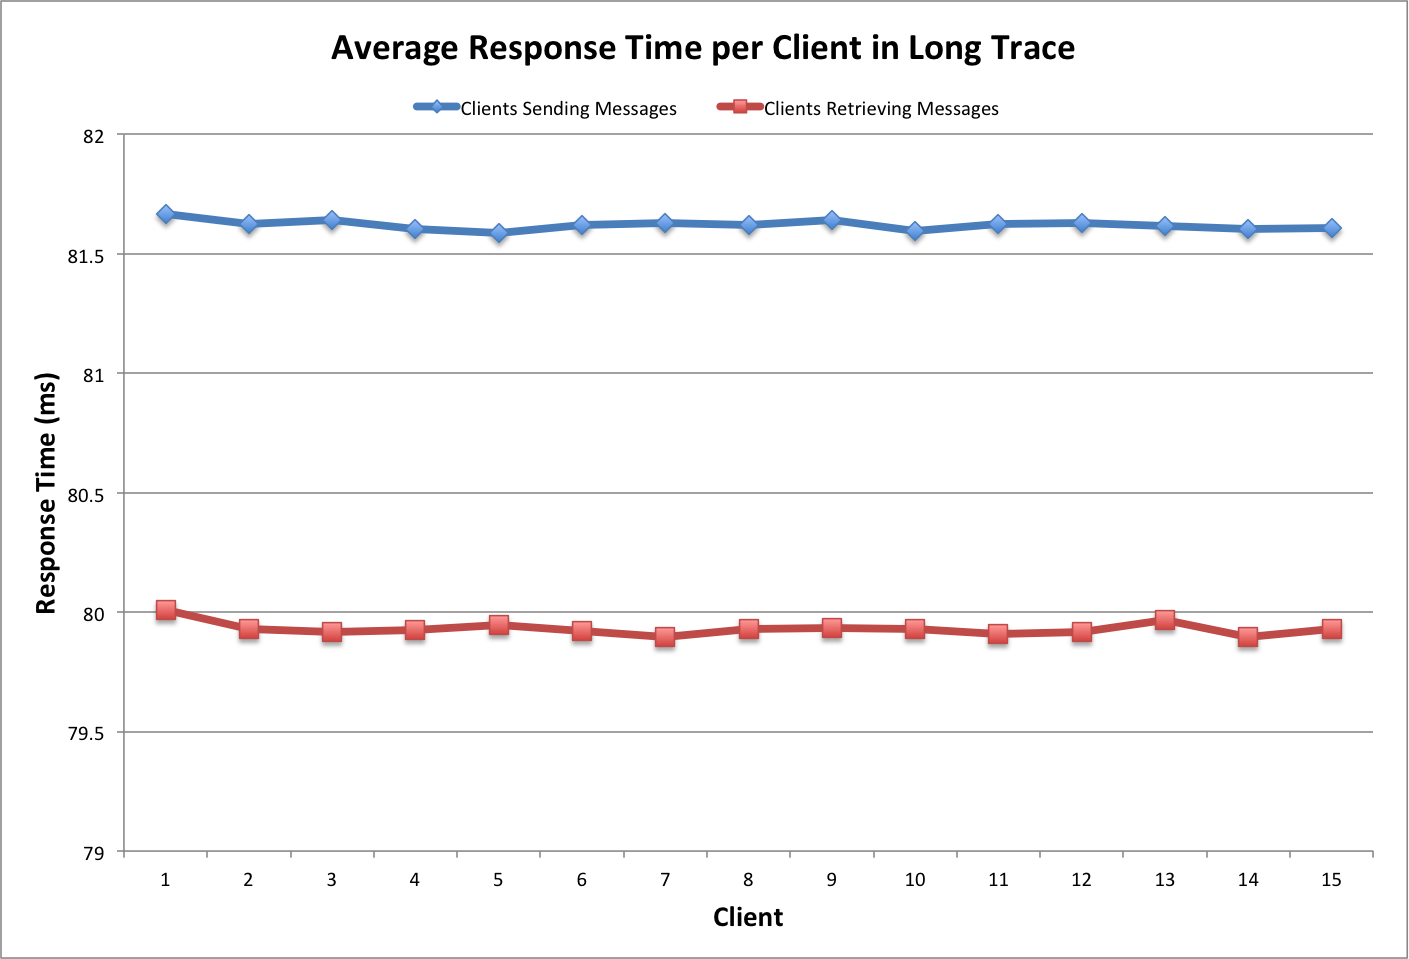
\includegraphics[scale=0.35]{stabilityRP.png}
	\caption{}
	\label{stabilityRP}
	%\input{soft-mmu-2.pdf}
\end{figure}
\begin{figure}[h!]
	\centering
	%\def \svgscale {\columnwidt}
	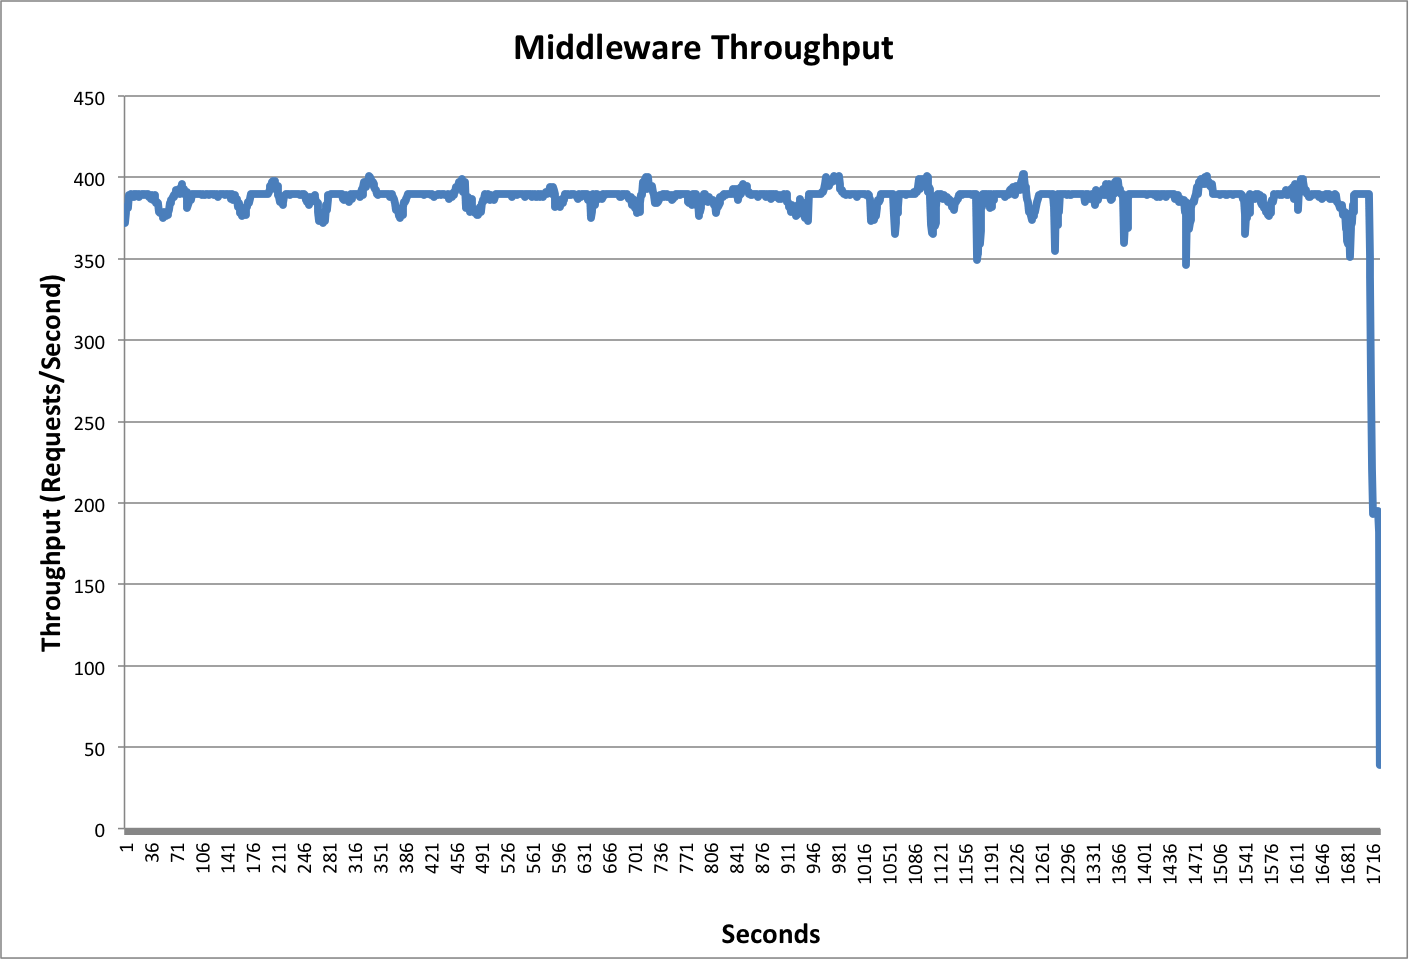
\includegraphics[scale=0.35]{stabilityTHR.png}
	\caption{}
	\label{stabilityTHR}
	%\input{soft-mmu-2.pdf}
\end{figure}
In order to perform a stability test the configuration of the system was the following, the database was already initialize it had 14750 messages stored; it had a size of 324MB. Two middleware node, one on each t2.medium instance, 15 clients connected to each middleware node, each group of 15 client were running in a t2.medium instance as well, which makes a total of 30 clients sending and receiving data. The period of running of the experiment was for 10 minutes and with 5 repetitions in total.\\

From the result plotted in Figures \ref{through} and \ref{stabilityTHR}, we can observe since the beginning a stable running since the warm-up face in the throughput of the system. In addition we can se the decrease of the throughput at the end in the cool down face. Furthermore there are some sparse down spikes in the throughput, which I point to effect of the java collector and the I/O activity in the middleware caused by the writing of the log files.\\

In addition to the analysis of the throughput we can observe the difference in response time in the two different operations being performed by the clients. Clearly the system take more time in create a new message and store it on the system than in retrieving a single message. This makes sense since when a message is about to be created it check if the queue where is going to be stored exist or not and if it doesn’t it creates that queue. This operation incurs in more time of processing then retrieving a single message.


\subsection{System Throughput}\label{sec:system-throughput}
For the Throughput analysis the configuration of the system was the following the same type and number of machines described in the system configuration are used. In order to find the maximum throughput increased the load in the system and the number of machines simultaneously.
\begin{figure}[h!]
	\centering
	%\def \svgscale {\columnwidt}
	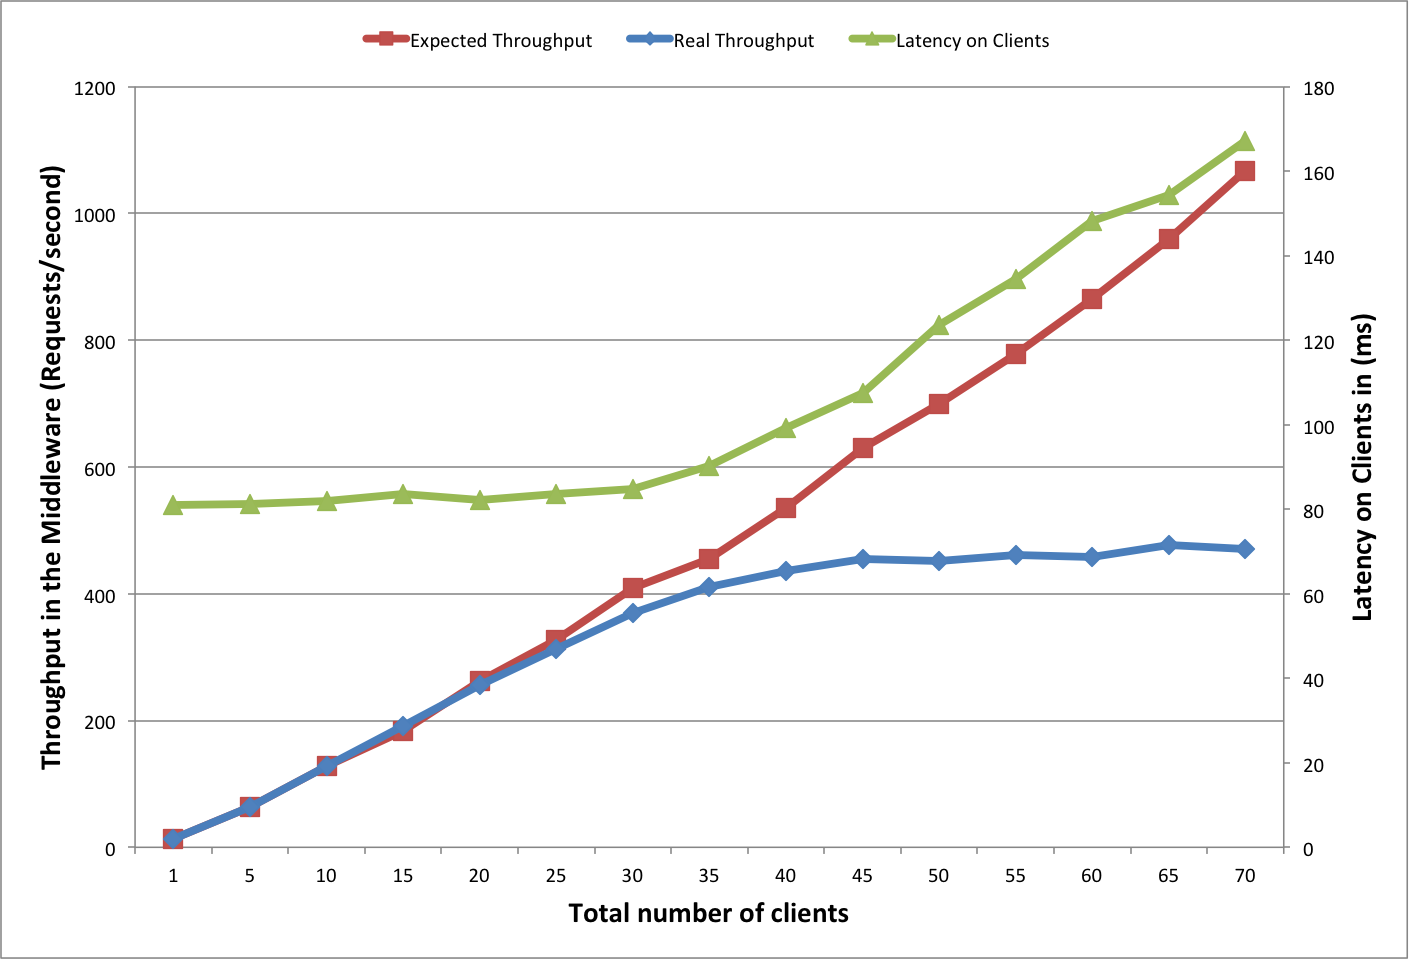
\includegraphics[scale=0.4]{through.png}
	\caption{}
	\label{through}
	%\input{soft-mmu-2.pdf}
\end{figure}

Assuming enough resources on my system I performed experiments with increments of five clients more on each middleware on each repetition. My hypothesis for this experiment was to observe a linear increase in the throughput and to observe a constant response time.\\

Nevertheless, given the results showed in Figure \ref{through} obtained after preforming constant increases for periods of ten minutes I was able to find the maximum throughput on my system. In addition I was able to observe the effect that the increment of load in the system affects the response time. In the figure I plotted what I expected to be the increment in the throughput. However when the middleware is handling more than forty clients the throughput stops increasing and remain more less constant. Nevertheless the Latency or average response time that the clients are having just continues increasing.\\

Even when the Middleware is configured to handle more clients with an initial configuration running a hundred Client Hanlders to attend the requests from clients, the response time increases because of the number of connections to the database, which in this experiment is fixed to 10, are not enough to satisfy the amount of operations the clients are requesting from the middleware. Since after each database operation a connection is being taken from the pool and when all the connections are occupied the client requests must wait until one connection gets free. This as consequence increases the response time in the clients.\\

Is important to mention that the data and plot reflect only one of the middleware and the response time of a single machine running clients. Nevertheless given the fact that in both machines the clients are preforming the same operation and both middleware have the exact same configuration the same analysis and results apply for the other components.

\subsection{System Scalability}\label{sec:system-scalability}

For the scalability tests I performed a scale-up and a scale out experiments. My hypothesis for these experiments was to expect the same behavior for both and observe a constant function measured metric response time or latency, in my clients.\\

In the scale up setting the configuration of my system was a single machine running client, one middleware machine with a middleware node and my database machine. The parameters I fixed in this experiment were the number clients with 15 clients, 5 Client Handlers in the middleware and 5 connections to the database in the middleware. The experiment was running for 10 minutes, and each client was running for 3 minutes and all the clients where sending new messages of 200 character to the system.\\

For the scaling setting I was increasing by the double the value of the parameters in my system. Therefore as part of my hypothesis I was expecting to see a double increment of my throughput in the system. The result of the scale up can be observer in the Table \ref{scaleup}.\\

\begin{table*}\centering
         % \ra{1.3}
         % \tabcolsep=0.5cm
         \scalebox{0.8}{
         \begin{tabular}{@{}cccc@{}}
                  \toprule
                  $Setting$ & 5 Client Handlers   & 10 Client Handlers & 20 Client Handler\\
                  
                  $/Metric$ & 15 Clients         & 30 Clients        & 60 Clients  \\
                  \cmidrule{2-4}
                 
			         Latency (ms)        & 80.22654714        & 80.25648836       & 81.48056189 \\
			         Throuhput (Req/sec) & 194.4534884        & 388.494186        & 766.6140351 \\
                  \bottomrule
                  \end{tabular}
         }
         \caption{}
         \label{scaleup}
 \end{table*}
 In the scaling out setting I wanted to achieve the same number with double incremental of my parameters. Therefore I used the same configuration for my 1 machine running clients, 1 middleware and 2 database running 15 clients, with 5 Client Handlers and 5 connections to the database and perform double value incremental having setting with 2 machines running clients, 2 middleware servers, then a final setting with 4 client machines, and 4 middleware server. Each single machine replicated was running with the same fixed value for the parameters, which were the mention previously. The result o the scale out setting can be observer in the Table \ref{scaleout}.\\
 
\begin{table*}\centering
         % \ra{1.3}
         % \tabcolsep=0.5cm
         \scalebox{0.8}{
         \begin{tabular}{@{}cccc@{}}
                  \toprule
                  $Setting$ & 1 Middleware	&2 Middlewares	&4 Middlewares\\
                  
                  $/Metric$ & 15 Clients         & 30 Clients        & 60 Clients  \\
                  \cmidrule{2-4}
					Latency (ms)&	80.22654714	&80.33796634	&81.48632835\\
					Throuhput (Req/sec)&	194.4534884	&388.3139535	&755.4543636\\
                  \bottomrule
                  \end{tabular}
         }
         \caption{}
         \label{scaleout}
 \end{table*} 
As I expect on my hypothesis my system on the scaling out setting was behaving like the scale up experiment. Nevertheless giving these scenarios, I consider scaling up factor is more efficient giving that the allocation of new requests to free connections is done by a single middleware which can be more efficient. However this may not be the case always since this depends in how the system is configured.\\

\subsection{Response Time Variations}\label{sec:response-time-variations}



\subsection{$2^k$ Experiment}\label{sec:k-experiment}
For the 2\^{}k experiment the two factors I decided to explore ere the number of concurrent client in my middleware (Handlers) and my number of connections in the database, the reason was because as I observed in my through put experiment by increasing the number of clients allowed in the system in the handler parameter the throughput was increasing. Furthermore I wanted to see the impact on the number of connection in the system.\\

Both parameters were explored in two levels each with the values of 10 and 20. As result I had to preform the experiment 4 times with adjusting the values of the previous parameters. Each experiment was running for 10 minutes, with t2.medium instances each client with and average workload of 12 requests per second.
By performing this experiment we are able to see the impact of these factors in the performance of the system in Request completed by second (Req/sec).

After the data seen in Table \ref{2k}, I define my two variables $x_{a}$ and $x_{b}$



\begin{table*}\centering
         % \ra{1.3}
         % \tabcolsep=0.5cm
         \scalebox{0.8}{
         \begin{tabular}{@{}rrcc@{}}
                  \toprule
                    & \multicolumn{3}{c}{Connection to Database} \\
                  \cmidrule{2-4}
                   \multicolumn{1}{c}{$Client Hanlder$} &&$10$ &$20$\\
                  \midrule 
			         10 &&$129.354782609$&$128.763478261$   \\
			          20 &&$257.597560976$&$258.93554007$   \\
                  \bottomrule
                  \end{tabular}
         }
         \caption{}
         \label{2k}
 \end{table*}  
 
 $$x_{a}=\begin{cases} -1& if\quad 10 \quad Connections\quad  to\quad  Dabatase\\1 & if\quad 20 \quad Connections\quad  to\quad  Dabatase\end{cases}\\
 $$
 $$x_{b}=\begin{cases} -1& if\quad 10 \quad Client\quad Hanlders\\1 & if\quad 20 \quad Client\quad Hanlders\end{cases}$$
 After the analysis of my result my hypothesis about the number of Client Handler impacting in high way the performance of my system is true. Furthermore I was able to show that given the current configuration of my database and the number of connections it has is more than enough for my system.\\
 
Furthermore my $2^k$ experiment show that the mean request per second is $193.6628405$, also the impact of the connection in request per second of my database connections is very low $ 0.186668686$ requests per second. However the value in my number of Client Handlers account for $ 64.60371004$ Requests per second. Finally the interaction of these two combined have an effect of $ 0.482320861$ Request per Second.See Table \ref{2kr}.


\begin{table*}\centering
         % \ra{1.3}
         % \tabcolsep=0.5cm
         \scalebox{0.8}{
         \begin{tabular}{@{}rrrrr@{}}
         \toprule
         
          & \multicolumn{3}{c}{Design of $2^2$ Experiment} \\
         \cmidrule{1-5}

         I           & A           & B           & AB          & y           \\
         \midrule 
         1           & -1          & -1          & 1           & 129.3547826 \\
         1           & 1           & -1          & -1          & 128.7634783 \\
         1           & -1          & 1           & -1          & 257.597561  \\
         1           & 1           & 1           & 1           & 258.9355401 \\
         774.6513619 & 0.746674746 & 258.4148402 & 1.929283442 & Total       \\
         193.6628405 & 0.186668686 & 64.60371004 & 0.482320861 & Total/4  \\
         \bottomrule  
         \end{tabular}
         }
         \caption{}
         \label{2kr}
         
 \end{table*}  

\subsection{Conclusion}\label{sec:conclusion}
